\section{Vysvětlete pojmy značka, abeceda, kód, prvek značky a symbol}
\begin{itemize}
    \item \textbf{Značka} je skupina prvků ze souboru \textbf{X}, která je přiřazena v procesu kódování jednomu prvku ze souboru \textbf{S}.
    \item \textbf{Abecedu} definujeme jako množinu používaných značek.
    \item \textbf{Kód} je soustava dohodnutých pravidel, podle kterých mají být tvořeny, přenášeny a vyhodnocovány značky, odpovídající daným znakům.
    \item \textbf{Prvek značky} je elementární část značky, prvek ze souboru X
    \item \textbf{Symbol} je interpretace značky nebo její částy v datovém signálu.
\end{itemize}

\section{Uveďte rozdíl mezi přenosovým kanálem a okruhem. Vysvětlete pojmy: komutovaný spoj, pevný spoj, simplexní, duplexní, poloduplexní spoj. Metody vytváření duplexního spojení}
\begin{itemize}
    \item \textbf{Přenosový kanál} - jde o soubor přenosových prostředků, který není přesně určen jen pro určitý druh přenosu, ale může být použit různými druhy přenosů využíván k  \textbf{jednosměrnůmu přenosu}.

    \item \textbf{Přenosový okruh} - Jde o soubor přenosových prostředků, který není přesně určen jen pro určitý druh přenosu, ale může být použit různými druhy přenosů využíván k \textbf{obousměrnému přenosu}.
    
    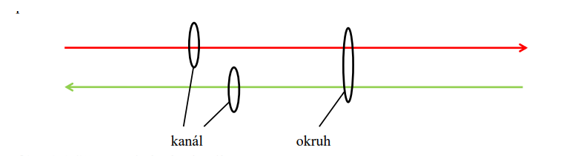
\includegraphics[]{images/okruh_kanal.png}
    
    \item \textbf{Komutovaný spoj} - jde o spoje, které se vytvoří před vlastním přenosem dat. př: spojení pomocí telefonních modemů nebo GPRS technologie.
    \item \textbf{Pevný spoj} - jde o trvalé spoje. Jejich nevýhoda spočívá ve snižování přenosové a spojovací kapacity systému vzhledem k ostatním uživatelům a proto je jejich realizace finančně náročná.
    \item \textbf{Simplexní spoje} - umožnují přenos signálu v jednom směru
    \item \textbf{Duplexní spoje} - umožnují současný přenos signálu v obou směrech
    \item \textbf{Poloduplexní spoje} - umožňují duplexní provoz, avšak pouze střídavě v jednom nebo druhém směru.
\end{itemize}
Metody realizace duplexního spojení
\begin{itemize}
    \item Kmitočtové
    \item Časové
    \item Obvodové
\end{itemize}

\section{Co jsou to provozní charakteristiky datavoých spojů. Popis nejčastěji užívaných}
\begin{itemize}
    \item \textbf{Přenosová rychlost} - potřebná rychlost závisí na potřebném objemu přenášených dat.
    Je odlišná na různých úrovních přenosu.
    Užitečná je někdy velmi výrazně nižší oproti udávané rychlosti fyzické.
    Dělí se dle dosažených maximálních rychlostí na malé, velké \dots.
    \item \textbf{Stálost přidělení spoje} - komutované a pevné.
    \item \textbf{Směr přenosu dat} - Podle směru rozlišujeme simplexní, duplexní a poloduplexní spoj.
    \item \textbf{Způsob přenosu značky}- podle časové realizace jednotlivých prvků rozlišujeme druhy přenosu
    \begin{itemize}
        \item \textbf{Paralelní způsob přenosu} - Všechny prvky značky se přenášejí ve stejném charakteristickém intervalu, po paralelních kanálech, kterých je stejný počet jako prvů ve značce.
        \item \textbf{Sériový způsob přenosu} - Prvky značky se přenášejí postupně za sebou po jednom kanálu.
        Tento způsob je náročný na čas poteřbný k přenosu značky.
                
    \end{itemize}
    \item \textbf{ Časový režim přenosu}- V přijímačy je nutno zajistit správné vyhodnocování značek, rozlišit jejich začátky a konec, tedy zajistit synchronizaci.
    Při sériovém přenosu se nejčastěji setkáme s těmito typy přenosu.
\end{itemize}

\section{Vysvětlete rozdíl mezi rychlostí přenosu a rychlostí přenosu informace}
\textbf{Přenosová rychlost} je definovaná jako počet dvojkových signálových prvků (bitů) přenesených za 1 s. [bit/s]

Rychlost přenosu informace - ???

\section{Vysvětlete pojmy časového režimu přenosu: synchronní přenos a arytmický. Uveďte příklady}
\begin{itemize}
    \item  \textbf{ Synchornní} - značky jsou vysílány kontinuálně a ke změně dochází po konstatním časovém intervalu.
    Není-li potřeba přenášet data přenáší se výplňové značky.
    \item \textbf{Arytmický} - vysílání může být zahájeno v jakémkoli okamžiku. 
    Počátek přenose se označuje specifická kombinace start a stop. Příkladem je rozhraní RS 232.
    
\end{itemize}

\section{Co je to systém přenosu dat. Jeho základní striktura a význam jednotlivých částí}
Jde o soubor podrobněji nespecifikovaných zařázení, které slouží k technické realizaci přenosu dat.
Tvoří jej hardware i software.

\includegraphics[]{images/přenos_dat.png}

\section{Specifikujte  4 základní typy rozhraní, které jsou zpravidla předmětem normalizace. Jaké znáte normalizační organizace}
\textbf{Typy rozhraní}
\begin{itemize}
    \item Mechanické vlastnosti
    \item Elektrické vlastnosti
    \item Funkční vlastnosti
    \item Operační vlastnosti
\end{itemize}
\textbf{Normalizační organizace}
\begin{itemize}
    \item ITU - International Telecommunication Union
     \item IEFT - Internet Engineering Task Force
     \item IEEE - Institute of Electrical and Electronic Engineering
     \item ANSI - American National Standards Institute
     \item ETSI - European Telecommunications Standards Institute
\end{itemize}

\section{Popište vlastnosti a použití rozhraní RS232 a USB}
\textbf{RS232}
\begin{itemize}
    \item Standardní sériové rozhraní, dříve používáno pro připojení telefonních modemů.
    Dnes se využívá pro malé přenosové rychlosti, konfigurační rozhraní atd.
    V mnoha technologiích je pro standardní podporu softwarově emulováné, ač je přenos realizován jinými technologiemi.
\end{itemize}
\textbf{USB}
\begin{itemize}
    \item Jde o sériové rozhraní, které se některých aplikacích nahrazuje dřive používané rozhraní.
    USB tvoří sběrnici s jedním zařízením typu Master a ostatní typu Slave.
    Můžeme se setkat s několika standardy:
\begin{itemize}
    \item Low speed
    \item Full speed
    \item High speed
    \item Super speed
\end{itemize}
\end{itemize}
\section{Ve kterých technologiích se můžete setkat s konektorem RJ45}
\begin{itemize}
    \item Rozhraní E1 - používané v telekomunikacích pro přenos 30 hovorových kanálů.
    \item Sériové rozhraní RS232 - viz. výše.
\end{itemize}
\section{Uveďte příklady sériových sběrnic pro mikrokontrolery}
\begin{itemize}
    \item I$^2$ C - Inter-integrated circiut - jde o sběrnici používající dvojice signálových vodičů v zapojení s otevřeným kolektorem SCLK a SDA
    \item SPI- Serial Peripheral Interface Bus - jde sběrnice využívající trojice signálů SCLK, MOSI a MISO
\end{itemize}